\section{The Implementation of Algorithms}
\subsection{Example of \( \mathbb{Z}_{17}[x]/(x^{8}-1) \)}

\begin{frame}
    \begin{itemize}
        \item We now demonstrate the actual implementations of the fast algorithm of 
        \[ \mathbb{Z}_{17}[x]/(x^{8}-1). \]
        We note that \( \omega_{4} = 4\) and \( \omega_{8} = 2 \).
        \item The first step is the projection:
        \begin{align*}
            \mathbb{Z}_{17}[x]/(x^{8}-1) &\underbrace{\cong}_{(1)} \mathbb{Z}_{17}[x]/(x^{4}-1) \times \mathbb{Z}_{17}[x]/(x^{4}+1) \\
            &\underbrace{\cong}_{(2)} \mathbb{Z}_{17}[x]/(x^{2}-1) \times \mathbb{Z}_{17}[x]/(x^{2}+1) \times \mathbb{Z}_{17}[x]/(x^{2}-4) \times \mathbb{Z}_{17}[x]/(x^{2}+4) \\
            &\underbrace{\cong}_{(3)} \mathbb{Z}_{17}[x]/(x-1) \times \mathbb{Z}_{17}[x]/(x+1) \times \mathbb{Z}_{17}[x]/(x-4) \times \mathbb{Z}_{17}[x]/(x+4) \\
            &\hspace{1cm} \times \mathbb{Z}_{17}[x]/(x-2) \times \mathbb{Z}_{17}[x]/(x+2) \times \mathbb{Z}_{17}[x]/(x-8) \times \mathbb{Z}_{17}[x]/(x+8).
        \end{align*}
        \item The input of the algorithm are two polynomials, and we will perform the projection on both of them.
        Let's denote a generic polynomial by \( a(x) \), and see how to implement the algorithm of such projection.

    \end{itemize}
\end{frame}

\begin{frame}
    \begin{itemize}
        \item Usually, the \emph{array} structure is used to represent a polynomial.
        If the input polynomial is \( a(x) = a_{0} + a_{1}x + \cdots + a_{7}x^{7} \), then the initial array representation is 
        \[ [a_{0}, a_{1}, \ldots, a_{7}]. \]
        \item The first layer projection is
        \[
            \mathbb{Z}_{17}[x]/(x^{8}-1) \underbrace{\cong}_{(1)} \mathbb{Z}_{17}[x]/(x^{4}-1) \times \mathbb{Z}_{17}[x]/(x^{4}+1) 
        \]
        \item It will project the polynomial \( a(x) \) to two polynomials:
        \begin{align*}
            a_{0} + a_{4} + (a_{1} + a_{5})x + (a_{2} + a_{6})x^{2} + (a_{3} + a_{7})x^{3} &\in \mathbb{Z}_{17}[x]/(x^{4} - 1)
            \intertext{and}
            a_{0} - a_{4} + (a_{1} - a_{5})x + (a_{2} - a_{6})x^{2} + (a_{3} - a_{7})x^{3} &\in \mathbb{Z}_{17}[x]/(x^{4} + 1)
        \end{align*}
        \item In our array representation, the projection is simply the addition and subtraction of the corresponding elements:
        \[ [a_{0}, a_{1}, a_{2}, a_{3}, a_{4}, a_{5}, a_{6}, a_{7}] \mapsto [a_{0} + a_{4}, a_{1} + a_{5}, a_{2} + a_{6}, a_{3} + a_{7}, a_{0} - a_{4}, a_{1} - a_{5}, a_{2} - a_{6}, a_{3} - a_{7}]. \]
    \end{itemize}
\end{frame}

\begin{frame}
    \begin{itemize}
        \item In our array representation, the projection is simply the addition and subtraction of the corresponding elements:
        \[ [a_{0}, a_{1}, a_{2}, a_{3}, a_{4}, a_{5}, a_{6}, a_{7}] \mapsto [a_{0} + a_{4}, a_{1} + a_{5}, a_{2} + a_{6}, a_{3} + a_{7}, a_{0} - a_{4}, a_{1} - a_{5}, a_{2} - a_{6}, a_{3} - a_{7}]. \]
        \item The pattern is not obvious, lets make a graph: 
        \begin{center}
            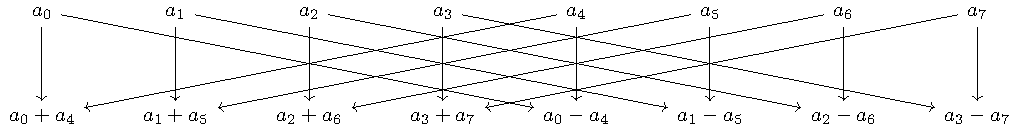
\includegraphics[width=0.8\textwidth]{tikzcd1.pdf} 
        \end{center}
        \item There are in fact four repeatitions of the same butterflies:
        \begin{center}
            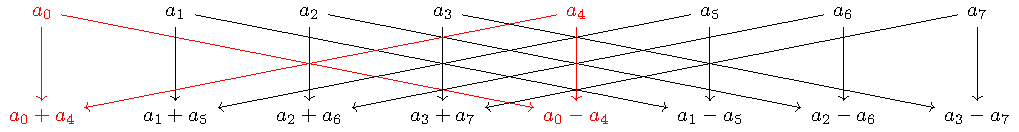
\includegraphics[width=0.8\textwidth]{tikzcd2.pdf} 
        \end{center}
    \end{itemize}
\end{frame}




\begin{frame}
    \begin{itemize}
        \item After implementing the first layer, we now focus on the second layer:
        \begin{align*}
            &\mathbb{Z}_{17}[x]/(x^{4}-1) \times \mathbb{Z}_{17}[x]/(x^{4}+1)\\
            &\quad\underbrace{\cong}_{(2)}\mathbb{Z}_{17}[x]/(x^{2}-1) \times \mathbb{Z}_{17}[x]/(x^{2}+1) \times \mathbb{Z}_{17}[x]/(x^{2}-4) \times \mathbb{Z}_{17}[x]/(x^{2}+4).
        \end{align*}
        \item Our array is now the output of the above layer (layer 1), we reset the symbols:
        \[ [a_{0}, a_{1}, a_{2}, a_{3}, a_{4}, a_{5}, a_{6}, a_{7}] \]
        which denotes \( a_{0} + a_{1}x + a_{2}x^{2} + a_{3}x^{3} \) and \(a_{4} + a_{5}x + a_{6}x^{2} + a_{7}x^{3}\) in the respective space.

        \item It will project two polynomials to four polynomials:
        \begin{align*}
            a_{0} + a_{2} + (a_{1} + a_{3})x &\in \mathbb{Z}_{17}[x]/(x^{2} - 1),\\
            a_{0} - a_{2} + (a_{1} - a_{3})x &\in \mathbb{Z}_{17}[x]/(x^{2} + 1),\\
            a_{4} + 4a_{6} + (a_{5} + 4a_{7})x &\in \mathbb{Z}_{17}[x]/(x^{2} - 4),\\
            a_{4} - 4a_{6} + (a_{5} - 4a_{7})x &\in \mathbb{Z}_{17}[x]/(x^{2} + 4).
        \end{align*}
        \item In our array representation, the projection is to perform:
        \[ 
        [a_{0}, a_{1}, a_{2}, a_{3}, a_{4}, a_{5}, a_{6}, a_{7}] \mapsto [a_{0} + a_{2}, a_{1} + a_{3}, a_{0} - a_{2}, a_{1} - a_{3}, a_{4} + 4a_{6}, a_{5} + 4a_{7}, a_{4} - 4a_{6}, a_{5} - 4a_{7}].
        \]

    \end{itemize}
\end{frame}


\begin{frame}
    \begin{itemize}
        \item In our array representation, the projection is to perform:
        \[ 
            [a_{0}, a_{1}, a_{2}, a_{3}, a_{4}, a_{5}, a_{6}, a_{7}] \mapsto [a_{0} + a_{2}, a_{1} + a_{3}, a_{0} - a_{2}, a_{1} - a_{3}, a_{4} + 4a_{6}, a_{5} + 4a_{7}, a_{4} - 4a_{6}, a_{5} - 4a_{7}].
        \]
    
        The pattern is not obvious, lets make a graph: 
        \begin{center}
            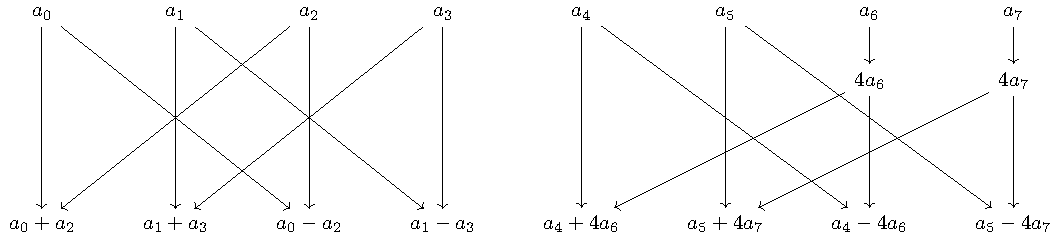
\includegraphics[width=0.8\textwidth]{tikzcd3.pdf}
        \end{center}

    \end{itemize}
\end{frame}

\begin{frame}
    \begin{itemize}
        \item After implementing the second layer, we now focus on the last layer:
        \begin{align*}
            &\mathbb{Z}_{17}[x]/(x^{2}-1) \times \mathbb{Z}_{17}[x]/(x^{2}+1) \times \mathbb{Z}_{17}[x]/(x^{2}-4) \times \mathbb{Z}_{17}[x]/(x^{2}+4)\\
            &\underbrace{\cong}_{(3)} \mathbb{Z}_{17}[x]/(x-1) \times \mathbb{Z}_{17}[x]/(x+1) \times \mathbb{Z}_{17}[x]/(x-4) \times \mathbb{Z}_{17}[x]/(x+4) \\
            &\hspace{1cm} \times \mathbb{Z}_{17}[x]/(x-2) \times \mathbb{Z}_{17}[x]/(x+2) \times \mathbb{Z}_{17}[x]/(x-8) \times \mathbb{Z}_{17}[x]/(x+8).
        \end{align*}
        \item Our array is now the output of the above layer (layer 2), we reset the symbols:
        \[ [a_{0}, a_{1}, a_{2}, a_{3}, a_{4}, a_{5}, a_{6}, a_{7}] \]


        \item It will project four polynomials to eight scalars:
        \begin{align*}
            a_{0} + a_{1} &\in \mathbb{Z}_{17}[x]/(x - 1),&
            a_{0} - a_{1} &\in \mathbb{Z}_{17}[x]/(x + 1),\\
            a_{2} + 4a_{3} &\in \mathbb{Z}_{17}[x]/(x - 4),&
            a_{2} - 4a_{3} &\in \mathbb{Z}_{17}[x]/(x + 4),\\
            a_{4} + 2a_{5} &\in \mathbb{Z}_{17}[x]/(x - 2),&
            a_{4} - 2a_{5} &\in \mathbb{Z}_{17}[x]/(x + 2),\\
            a_{6} + 8a_{7} &\in \mathbb{Z}_{17}[x]/(x - 8),&
            a_{6} - 8a_{7} &\in \mathbb{Z}_{17}[x]/(x + 8).
        \end{align*}
        \item In our array representation, the projection is to perform:
        \[ 
        [a_{0}, a_{1}, a_{2}, a_{3}, a_{4}, a_{5}, a_{6}, a_{7}] \mapsto 
        [a_{0} + a_{1}, a_{0} - a_{1}, a_{2} + 4a_{3}, a_{2} - 4a_{3}, a_{4} + 2a_{5}, a_{4} - 2a_{5}, a_{6} + 8a_{7}, a_{6} - 8a_{7}].
        \]


    \end{itemize}
\end{frame}

\begin{frame}
    \begin{itemize}
        \item In our array representation, the projection is to perform:
        \[ 
        [a_{0}, a_{1}, a_{2}, a_{3}, a_{4}, a_{5}, a_{6}, a_{7}] \mapsto 
        [a_{0} + a_{1}, a_{0} - a_{1}, a_{2} + 4a_{3}, a_{2} - 4a_{3}, a_{4} + 2a_{5}, a_{4} - 2a_{5}, a_{6} + 8a_{7}, a_{6} - 8a_{7}].
        \]
    
        The pattern is not obvious, lets make a graph: 
        \begin{center}
            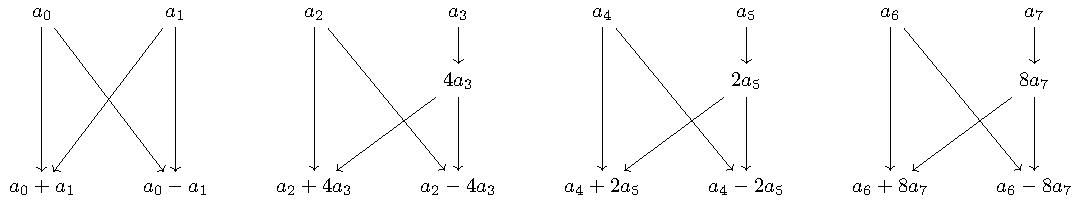
\includegraphics[width=0.8\textwidth]{tikzcd4.pdf}
        \end{center}
        

    \end{itemize}
\end{frame}

\begin{frame}
    In total, the projection can be represented by the following graph:
    \begin{center}
        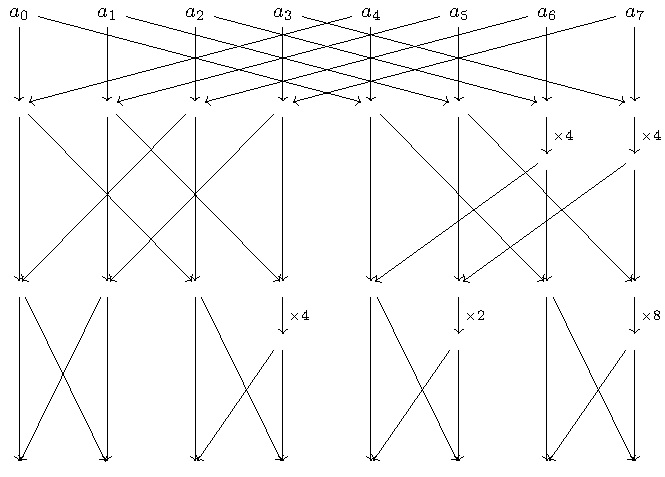
\includegraphics[width=0.7\textwidth]{tikzcd5.pdf}
    \end{center}
\end{frame}

\begin{frame}
    \begin{itemize}
        \item Ok! After the projection, the point-wise multiplication is simple. 
        \item The remark I want to make here is that, during the whole process, the multiplication is performed modulo \( 17 \). 
        Such modulus multiplication (mod-mul for short) is a time-consuming operation.
        \item To deal with this, mathematicians invented various \emph{reduction algorithms}, e.g., Barrett reduction, Montgomery reduction, Plantard reduction etc.
        \item The choice of reduction algorithm depends on many factors, including the machine architecture, the parallelization, etc.
        \item There is a review in the following paper:

    \end{itemize}
\end{frame}

\begin{frame}
\begin{itemize}
    \item Finally, we have to rebuild the polynomial from the output of the last layer.
    \item Note that the rebuiding is the inverse of the projection, so we can rebuild the polynomial according to the graph, but you should look it conversely:
    \begin{center}
        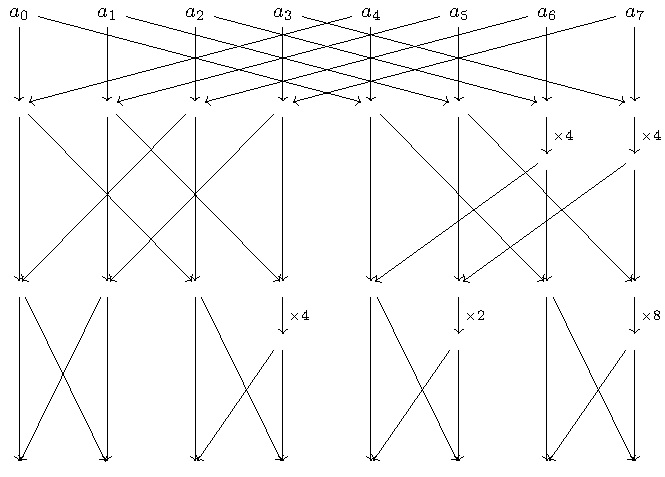
\includegraphics[width=0.6\textwidth]{tikzcd5.pdf}
    \end{center}
\end{itemize}
\end{frame}
